\begin{frame}{Experiment 4}
\setbeamercovered{invisible}
\fontsize{12pt}{15}\selectfont
\only<1>{{\large\textbf{Learning transfer from syntactic training in language to tool use}}\\
Testing the \textbf{reverse learning transfer}: training syntactic processes with complex sentences should \textbf{improve tool use}.}
\pause

\only<2>{{\large\textbf{Experimental design:}}
\begin{itemize}
    \item Measuring \textbf{tool-use performance} after syntactic training.
    \item Type of training \textbf{clause} was \textbf{randomly assigned} (unknown to experimenter).
    \item Before and after training, they \textbf{calculated the number of pegs} entered with the tool.
\end{itemize}}
\pause
\only<3>{
\begin{figure}
    \centering
    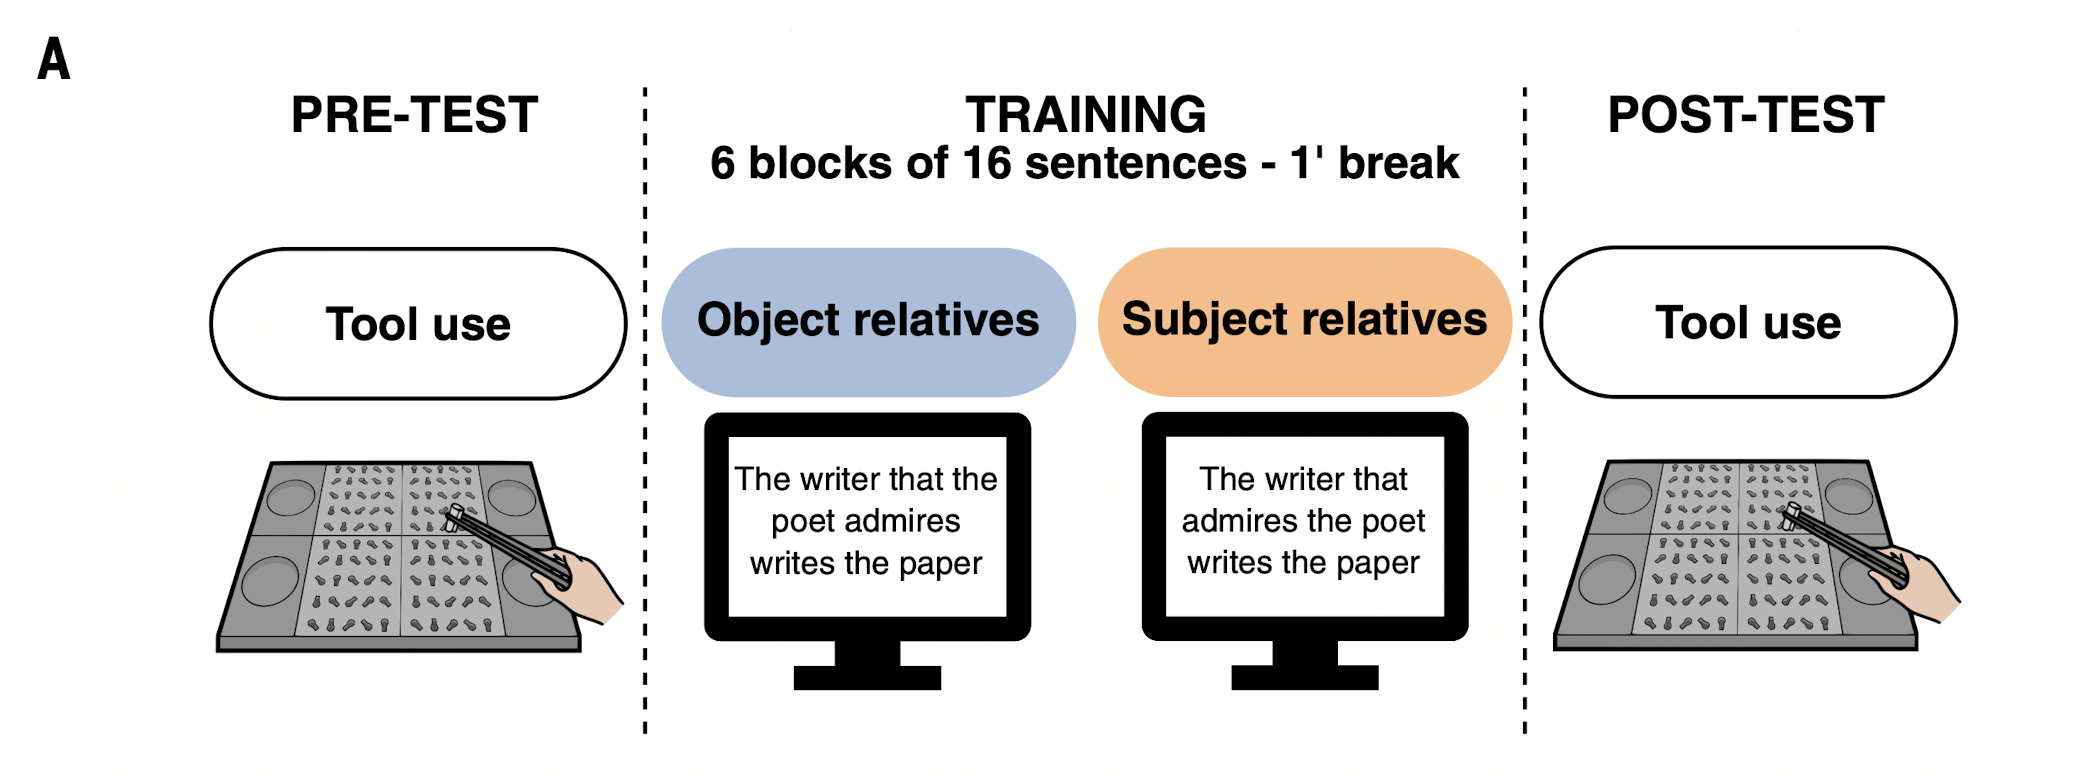
\includegraphics[width=11cm]{images/paper_pics/fig4A.png}
    %\caption*{}
    \label{fig:label10}
\end{figure}
}

\end{frame}
